\section{Sessão 1}

Na primeira sessão, serão montadas duas secções biquadráticas de 3 Amplificadores Operacionais (AmpOp). Em particular, será estudada uma secção biquadrática Kerwin, Huelsman e Newcom (KHN) e Tow-Thomas (TT). Estes filtros são compostos por circuitos elementares mais simples, alguns deles apresentados na Fig.~\ref{fig:circuitosElemnatres}. As relações entre a entrada e a saída destes circuitos elementares podem ser obtidas através de técnicas elementares de análise de circuitos. Dado serem bem conhecidas, as suas relações entrada saída são apresentadas sem análise. Temos, para o circuito subtractor
\begin{equation}\label{eq:subtartor}
    V_o(s)=-\frac{R_4}{R_1}V_1(s) +\left(1+\frac{R_4}{R_1}\right)\frac{R_3}{R_2+R_3}V_2(s)\:,
\end{equation}
para o circuito somador-inversor\label{eq:sum_inv}
\begin{equation}
    V_o(s)= -\frac{R_3}{R_1}V_1(s) -\frac{R_3}{R_2}V_2(s)\:,
\end{equation}
para o circuito multiplicador-inversor 
\begin{equation}\label{eq:multInv}
    \frac{V_o(s)}{V_i(s)} = -\frac{R_2}{R_1}\:,
\end{equation}
e para o integrador inversor
\begin{equation}\label{eq:int_inv}
    \frac{V_o(s)}{V_i(s)} = -\frac{1}{RCs}\:.
\end{equation}

\begin{figure}[h!]
    \centering
    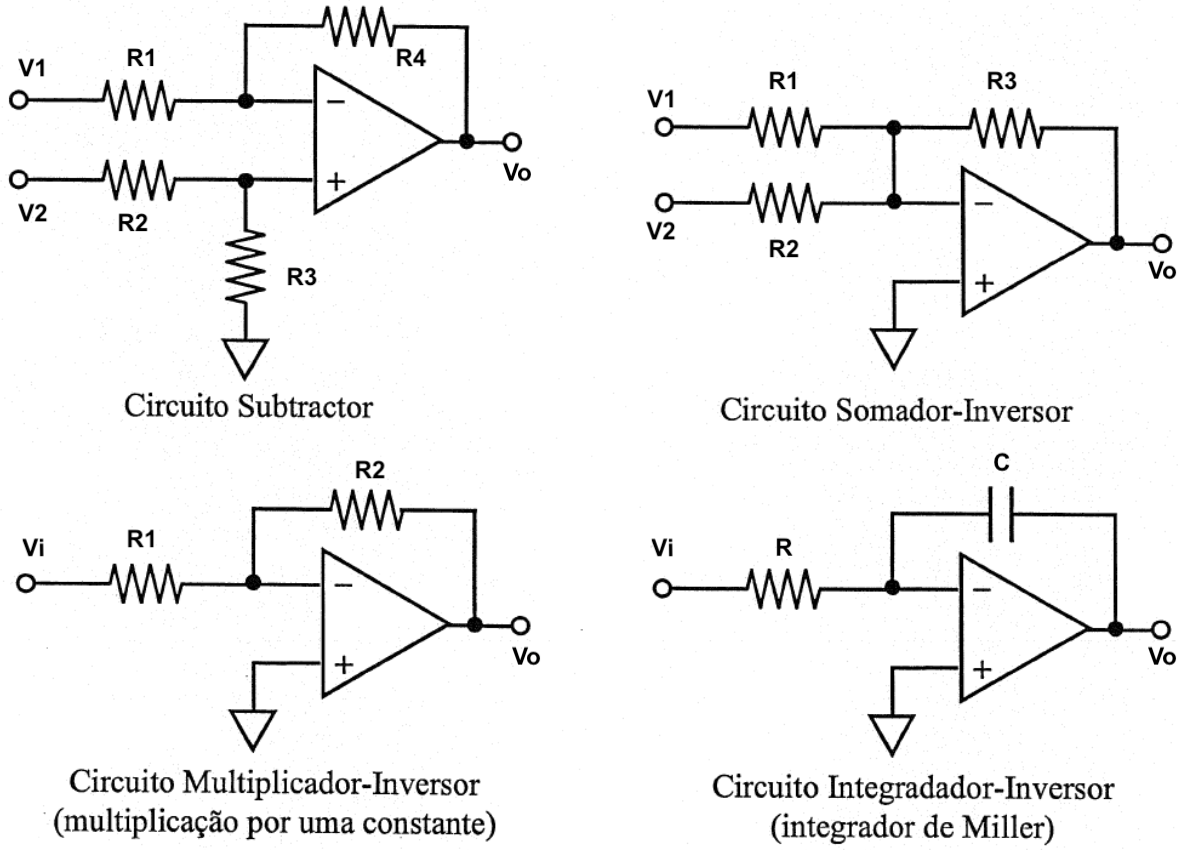
\includegraphics[width = 0.8\textwidth]{Imagens/circuitosElementares.png}
    \caption{Circuito eletrónicos elementares.}
    \label{fig:circuitosElemnatres}
\end{figure}

\subsection{Secção biquadrática KHN}

\subsubsection{Análise Teórica}
A resposta de uma secção biquadrática pode ser modelada por uma equação diferencial de 2º grau, de coeficientes constantes, que pode ser convenientemente descrita por um diagrama de fluxo de sinal (DFS) representado em função da variável complexa $s = j\omega$. Para o DFS da Fig. \ref{fig:dfs_KHN}, que permite modelar uma secção biquadrática de KHN, são facilmente obtidas as seguintes relações
\begin{equation}\label{eq:relacoesKHN}
    \begin{cases}
    V_1(s) = K V_i(s) + V_2(s)/Q - V_3(s) \\
    V_2(s) = -\omega_0 V_1(s)/s\\
    V_3(s) = -\omega_0 V_2(s)/s
    \end{cases}\:.
\end{equation}
Resolvendo o sistema de equações \eqref{eq:relacoesKHN} em ordem a $V_1(s), V_2(s)$, e $V_3(s)$, obtêm-se as funções transferência
\begin{equation}\label{eq:tfKHN}
\begin{split}
    T_1(s) = \frac{V_1(s)}{V_i(s)} =\frac{Ks^2}{s^2+(\omega_0/Q)s+\omega_0^2}\:, \\ 
    T_2(s) = \frac{V_2(s)}{V_i(s)} =\frac{-K\omega_0 s}{s^2+(\omega_0/Q)s+\omega_0^2}\:, \\
    T_3(s) = \frac{V_3(s)}{V_i(s)} =\frac{K\omega_0^2}{s^2+(\omega_0/Q)s+\omega_0^2} \:.
    \end{split}
\end{equation}
Como seria de esperar todas as funções transferência são de 2ª ordem, pelo que têm dois pólos. Em primeiro lugar, $T_1(s)$ tem dois zeros na origem, ganho estático nulo, \textit{i.e.}, $\lim_{\omega \rightarrow 0} T_1(j\omega) = 0$, e degenera num ganho constante para altas frequências, \textit{i.e.}, $\lim_{\omega \rightarrow \infty} T_1(j\omega) = K$. Por estas razões, $T_1(s)$ é passa-alto. Em segundo lugar, $T_2(s)$ tem um zero na origem, ganho estático nulo, \textit{i.e.}, $\lim_{\omega \rightarrow 0} T_2(j\omega) = 0$, e atenua as altas frequências, \textit{i.e.}$, \lim_{\omega \rightarrow \infty} T_2(j\omega) = 0$. Por estas razões, $T_2(s)$ é passa-banda. Em terceiro lugar, $T_2(s)$ não tem zeros, tenho ganho estático não nulo, \textit{i.e.}, $\lim_{\omega \rightarrow 0} T_2(j\omega) = K$, e atenua as altas frequências, \textit{i.e.}, $\lim_{\omega \rightarrow \infty} T_2(j\omega) = 0$. Por estas razões, $T_3(s)$ é passa-baixo. 

\begin{figure}
    \centering
    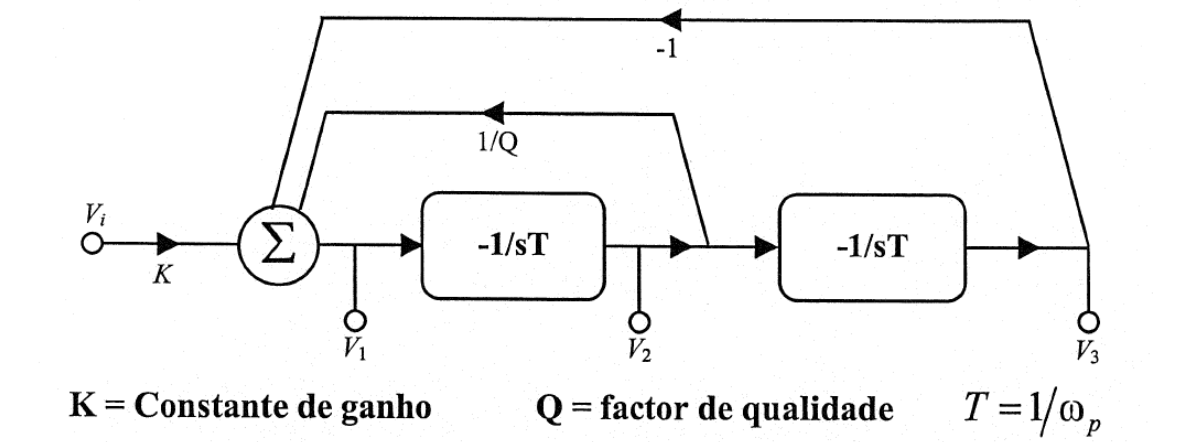
\includegraphics[width = 0.8\textwidth]{Imagens/dfs.png}
    \caption{Diagrama de fluxo de sinal da secção biquadrática KHN.}
    \label{fig:dfs_KHN}
\end{figure}

É de notar que como o denominador é comum às três funções de transferência, ou seja, têm os mesmo pólos, as características da resposta transiente dos 3 filtros será semelhante. Primeiro, a frequência de corte dos filtros passa-alto e passa-banda é igual a $\omega_0$ que também corresponde à frequência central do filtro passa-banda. Segundo, o fator de qualidade $Q$ e o ganho $K$ são também comuns a todos os filtros. Terceiro, os filtros passa-alto e passa-baixo atingem o mesmo ganho máximo. Quarto, na região de corte (a altas frequências para o passa-baixo e a baixas frequências para o passa-alto) o ganho varia assimptoticamente a $40$dB/dec. Já no caso das duas regiões de corte do passa-banda (a altas e baixas frequências) verifica-se que esta variação é de $20$dB/dec.

Consideremos, agora, o esquema eléctrico da implementação de uma secção biquadrática KHN, apresentado na Fig. \ref{fig:KHN}. Analisando o circuito, fazendo uso do circuito elementar integrador-inversor \eqref{eq:int_inv}, é possível estabelecer
\begin{equation}\label{eq:condKNHw0}
V_2(s) = -\frac{1}{R_6C_1}V_1(s)\:,\quad \quad \quad V_3(s) = -\frac{1}{R_{11}C_2}V_2(s) 
\end{equation}
e, por comparação com as duas primeiras equações de \eqref{eq:relacoesKHN}, vem que 
\begin{equation}\label{eq:w0khn}
\omega_0 = \frac{1}{R_6C_1}= \frac{1}{R_{11}C_2}.
\end{equation}
Para além disso, utilizando o teorema da sobreposição e o circuito elementar subtractor \eqref{eq:subtartor}, obtém-se
\begin{equation}
V_1(s) =\frac{P_2}{R_3+P_2}\left(1+\frac{R_5}{R_2}\right) V_i(s) + \frac{R_3}{R_3+P_2}\left(1+\frac{R_5}{R_2}\right) V_2(s)  -\frac{R_5}{R_2}V_3(s)\:.
\end{equation}
Assim, por comparação com a terceira equação de \eqref{eq:relacoesKHN}, é possível obter uma expressão para o ganho 
\begin{equation}\label{eq:Kkhn}
    K=\frac{P_2}{R_3+P_2}\left(1+\frac{R_5}{R_2}\right)\:,
\end{equation}
para o fator de qualidade
\begin{equation} \label{eq:Qkhn}
    \frac{1}{Q}=\frac{R_3}{R_3+P_2}\left(1+\frac{R_5}{R_2}\right) \Rightarrow Q = \frac{R_3+P_2}{R_3\left(1+\frac{R_5}{R_2}\right)}\:,
\end{equation}
e tem que se verificar 
\begin{equation}\label{eq:condKHN}
    -\frac{R_5}{R_2} = -1 \Rightarrow R_5 = R_2
\end{equation}
para que seja possível modelar a secção biquadrática KHN da Fig. \ref{fig:KHN} através do DFS da Fig \ref{fig:dfs_KHN}. Substituindo os valores dos componentes indicados em \eqref{eq:w0khn}, \eqref{eq:Kkhn}, e \eqref{eq:Qkhn} obtemos os valores teóricos de $\omega_0$, $K$ e $Q$ dos filtros utilizados na atividade laboratorial, apresentados na Tabela \ref{tab:parKHN}. Verifica-se, ainda, que a condição \eqref{eq:condKHN} é verificada.

\begin{figure}[h!]
    \centering
    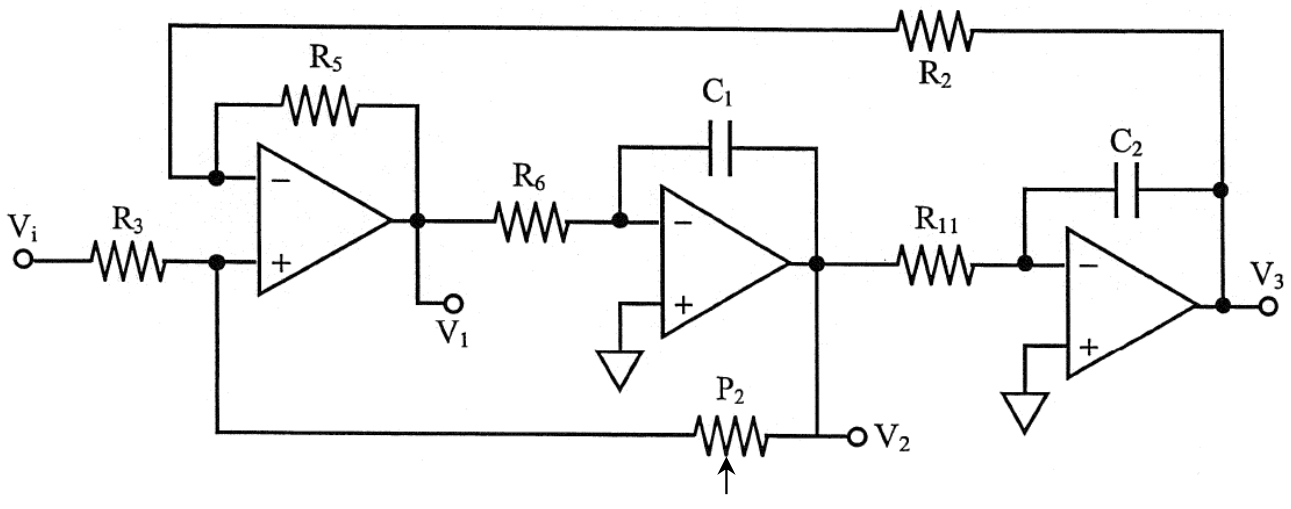
\includegraphics[width = 0.8\textwidth]{Imagens/KHN.png}
    \caption{Secção biquadrática KHN.}
    \label{fig:KHN}
\end{figure}

\begin{table}[h!]
    \centering
     \caption{Valores teóricos de $\omega_0$, $K$ e $Q$ dos filtros, arredondados a 4 algarismos significativos.}
    \begin{tabular}{cccc}
        \hline
         $\omega_0$ & $f_0$ & $Q$ & $K$ \\
         \hline
         $2.128 \times 10^{4}$ rad/$\mathrm{s^{-1}}$ & 3.386 kHz & 1.000 & 1.000\\
          \hline
    \end{tabular}
   
    \label{tab:parKHN}
\end{table}

Numa segunda instância a configuração da secção biquadrática KNH foi alterada de acordo com o esquema apresentado na Fig. \ref{fig:KNH_pot}, em que se pode agora fazer variar a resistência do potenciómetro, em vez de o usar como uma resistência de valor constante como anteriormente. Designando as resistências do potenciómetro entre o terminal móvel e os extremos como $R_g$ e $R_v$, como indicado na Fig. \ref{fig:KNH_pot}, vem 
\begin{equation}
    R_v + R_g = P_2\:.
    \label{eq:rv_rg}
\end{equation}

\begin{figure}[h!]
    \centering
    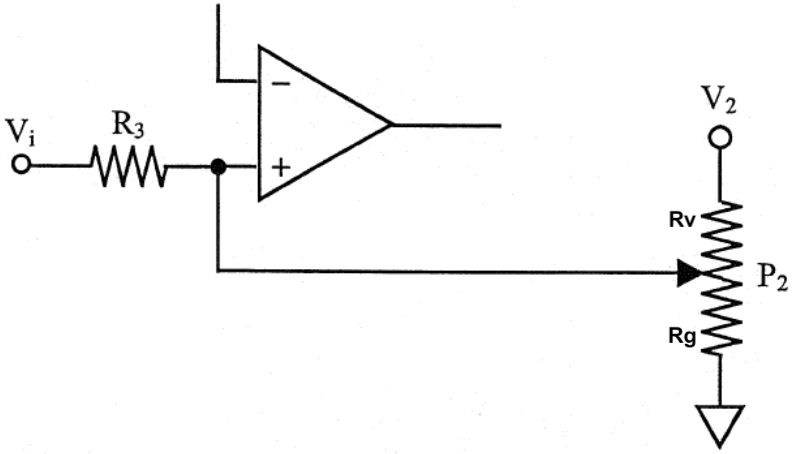
\includegraphics[width = 0.6\textwidth]{Imagens/KNH_pot.png}
    \caption{Alteração de configuração da secção biquadrática KHN.}
    \label{fig:KNH_pot}
\end{figure}

É fácil verificar que, com a nova configuração, \eqref{eq:condKNHw0} permanece válida, pelo que $\omega_0$ é dado por \eqref{eq:w0khn} e permanece inalterado. Recalculando o circuito elementar subtractor \eqref{eq:subtartor} presente neste filtro e fazendo uso do teorema da sobreposição para a nova configuração, obtém-se
\begin{align*}
        V_1(s) =&\frac{R_v||R_g}{R_3+R_v||R_g}\left(1+\frac{R_5}{R_2}\right) V_i(s) + \frac{R_3||R_g}{R_3||R_g+P_2}\left(1+\frac{R_5}{R_2}\right) V_2(s)  -\frac{R_5}{R_2}V_3(s)\\
=&\frac{(P_2-R_g)R_g}{R_3P_2+(P_2-R_g)R_g}\left(1+\frac{R_5}{R_2}\right) V_i(s) + \frac{R_3||R_g}{R_3||R_g+P_2}\left(1+\frac{R_5}{R_2}\right) V_2(s)  -\frac{R_5}{R_2}V_3(s)\:.
\end{align*}
Assim, por comparação com a terceira equação de \eqref{eq:relacoesKHN}, é possível obter uma nova expressão para o ganho 
\begin{equation}\label{eq:KkhnPot}
    K=\frac{(P_2-R_g)R_g}{R_3P_2+(P_2-R_g)R_g}\left(1+\frac{R_5}{R_2}\right)\:,
\end{equation}
para o fator de qualidade
\begin{equation} \label{eq:QkhnPot}
    \frac{1}{Q}= \frac{R_3||R_g}{R_3||R_g+P_2}\left(1+\frac{R_5}{R_2}\right) \Rightarrow Q = \frac{R_3||R_g+P_2}{(R_3||R_g)\left(1+\frac{R_5}{R_2}\right)}\:,
\end{equation}
e tem que se verificar \eqref{eq:condKHN}. Utilizando \eqref{eq:KkhnPot} e \eqref{eq:QkhnPot} é possível representar graficamente a evolução de $K$ e de $Q$ com a posição do potenciómetro. As evoluções destes dois parâmetros são apresentadas na Fig. \ref{fig:KQpot}. Primeiro, notamos que o ganho decresceu para valores cerca de uma ordem de grandeza abaixo do ganho unitário da configuração estudada anteriormente. Segundo, é de salientar que o ganho para $R_g = R$ é igual ao ganho para $R_g = P_2-R$, com $R \in [0;P_2]$. Esta propriedade é verificada experimentalmente, como detalhado na Secção \ref{sec:KNH_exp}. Terceiro, notamos que para valores baixos de $R_g$, $Q$ toma valores muito elevados, de facto, no limite $\lim_{R_g \rightarrow 0} Q = +\infty$ e os pólos dos filtros deslocam-se para o eixo imaginário. À medida que se aumenta $R_g$, $Q$ decresce monotonamente segundo uma hipérbole.

\begin{figure}[ht]
     \begin{subfigure}[b]{0.48\textwidth}
         \centering
         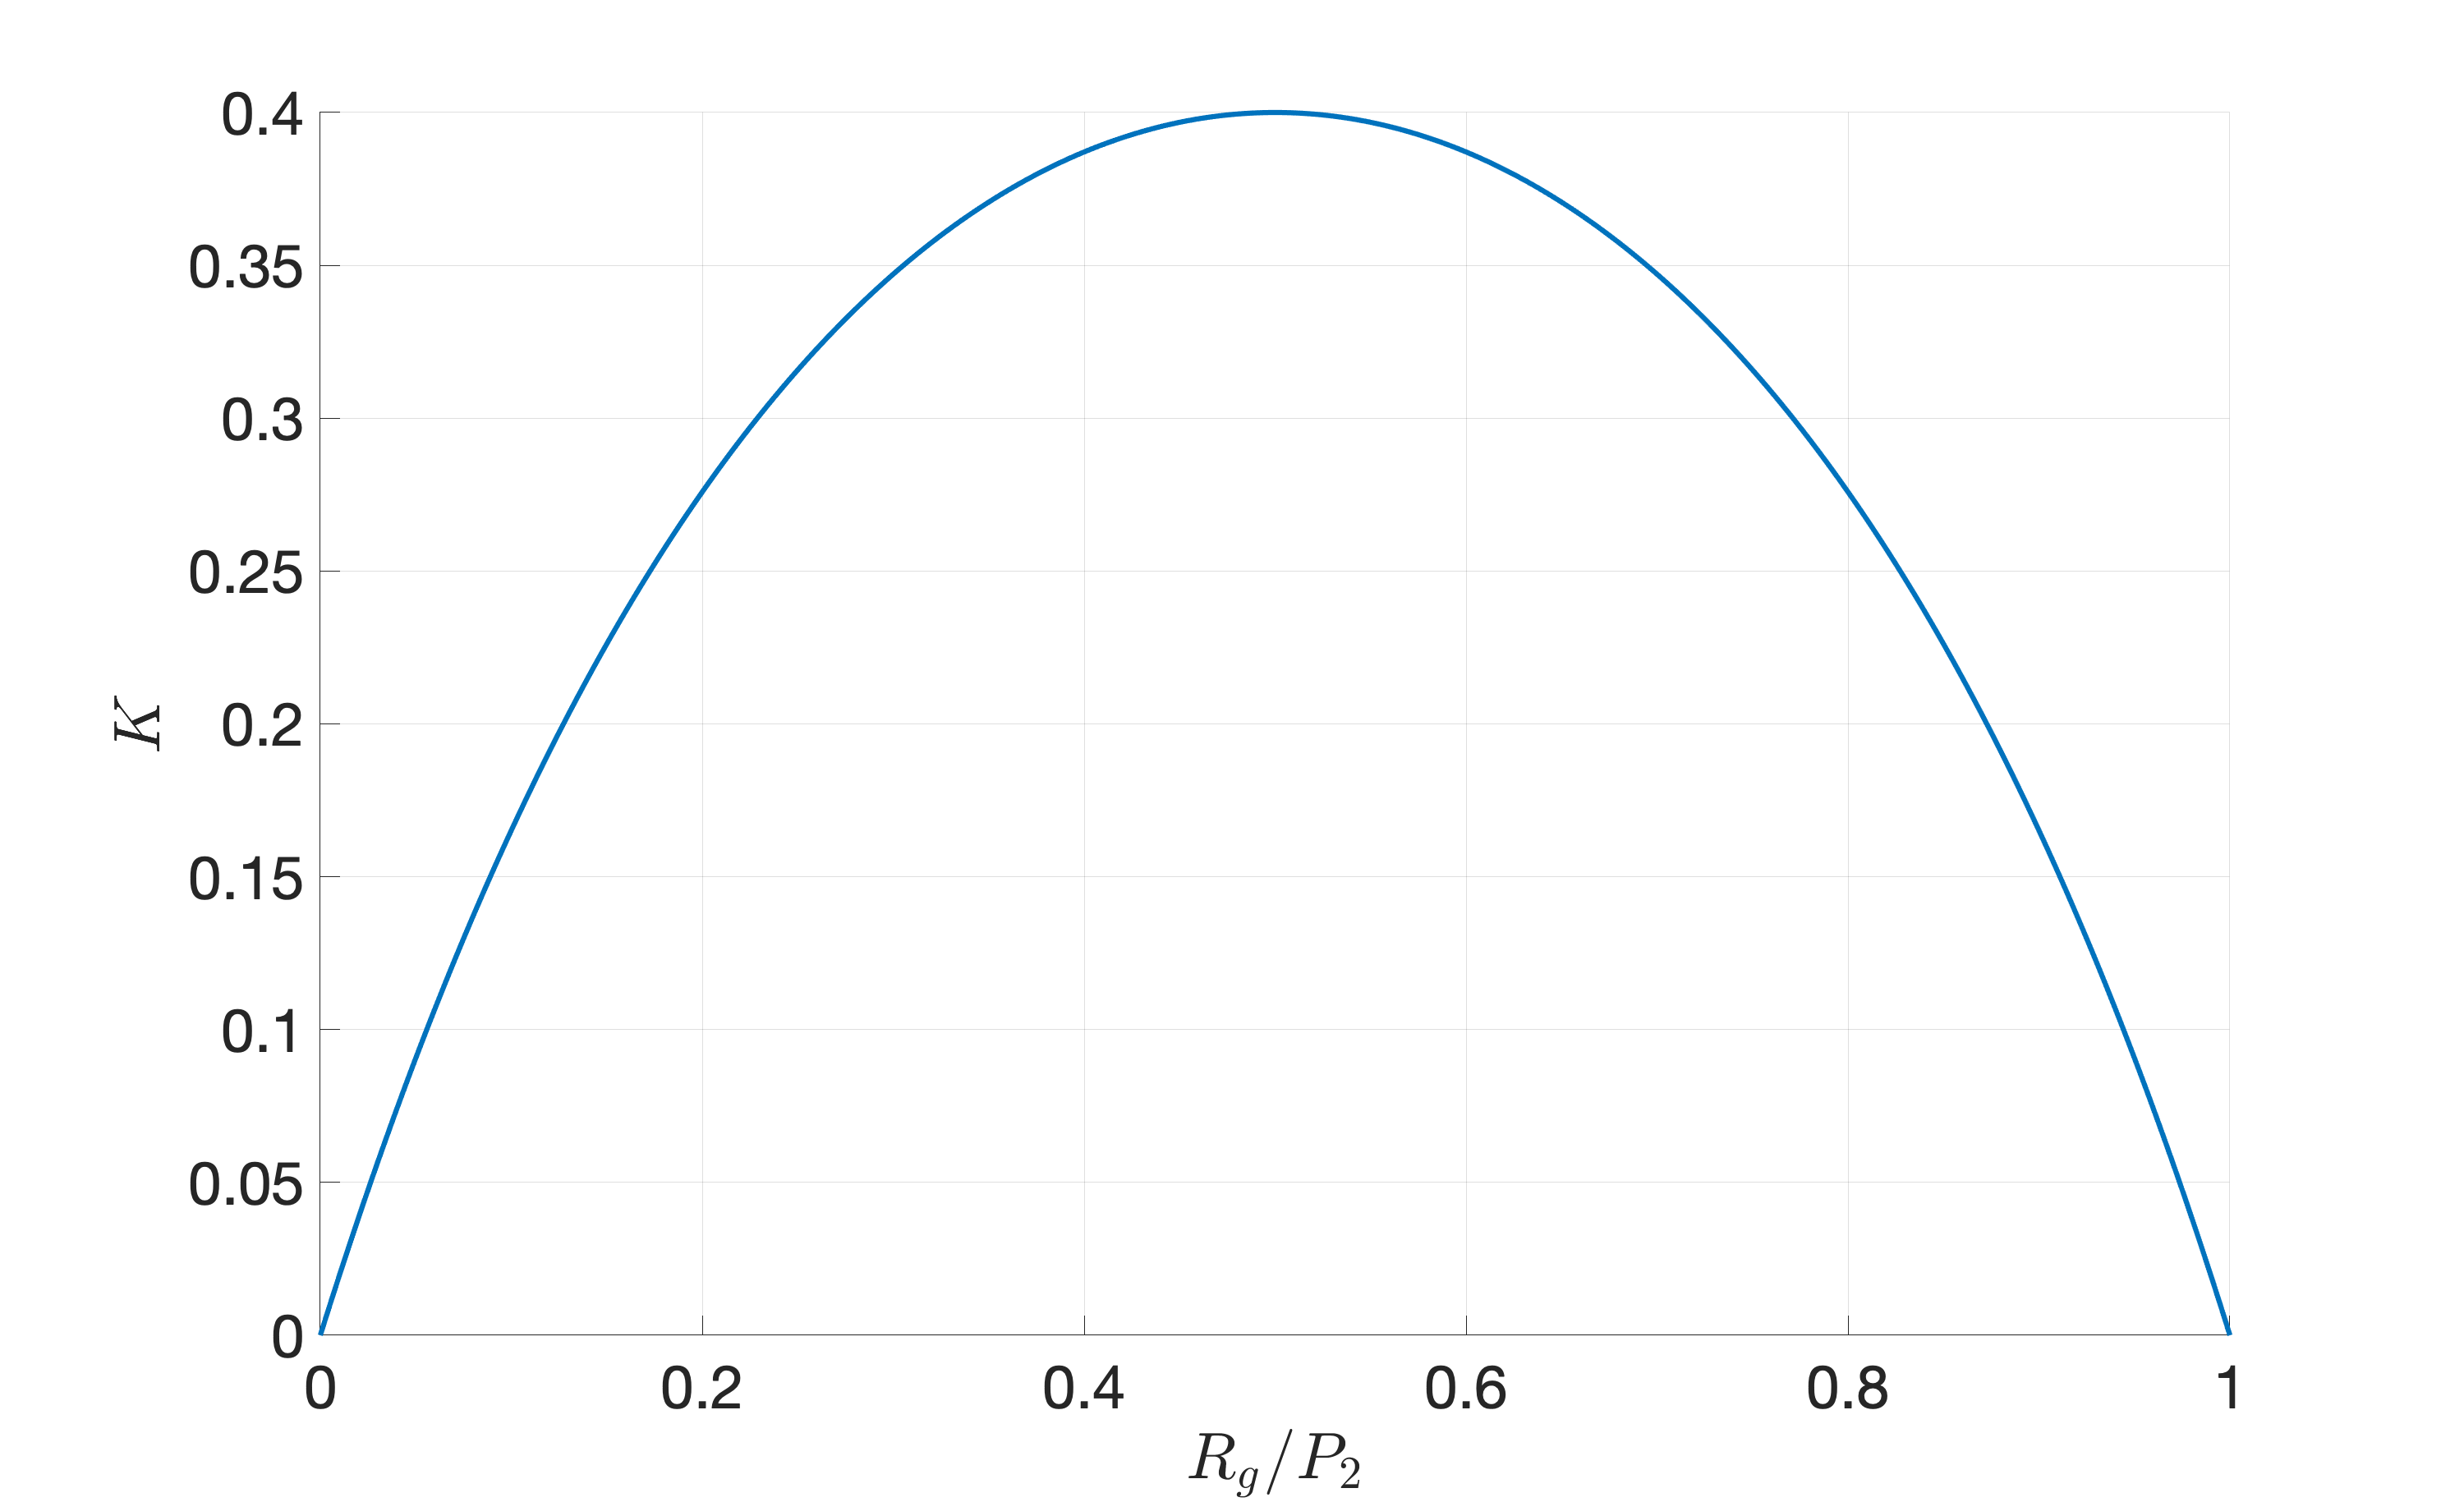
\includegraphics[width=\textwidth]{Imagens/1_5_6_GainPotentiometer3.png}
         \caption{Evolução de $K$.}
     \end{subfigure}
     \hfill
     \begin{subfigure}[b]{0.48\textwidth}
         \centering
         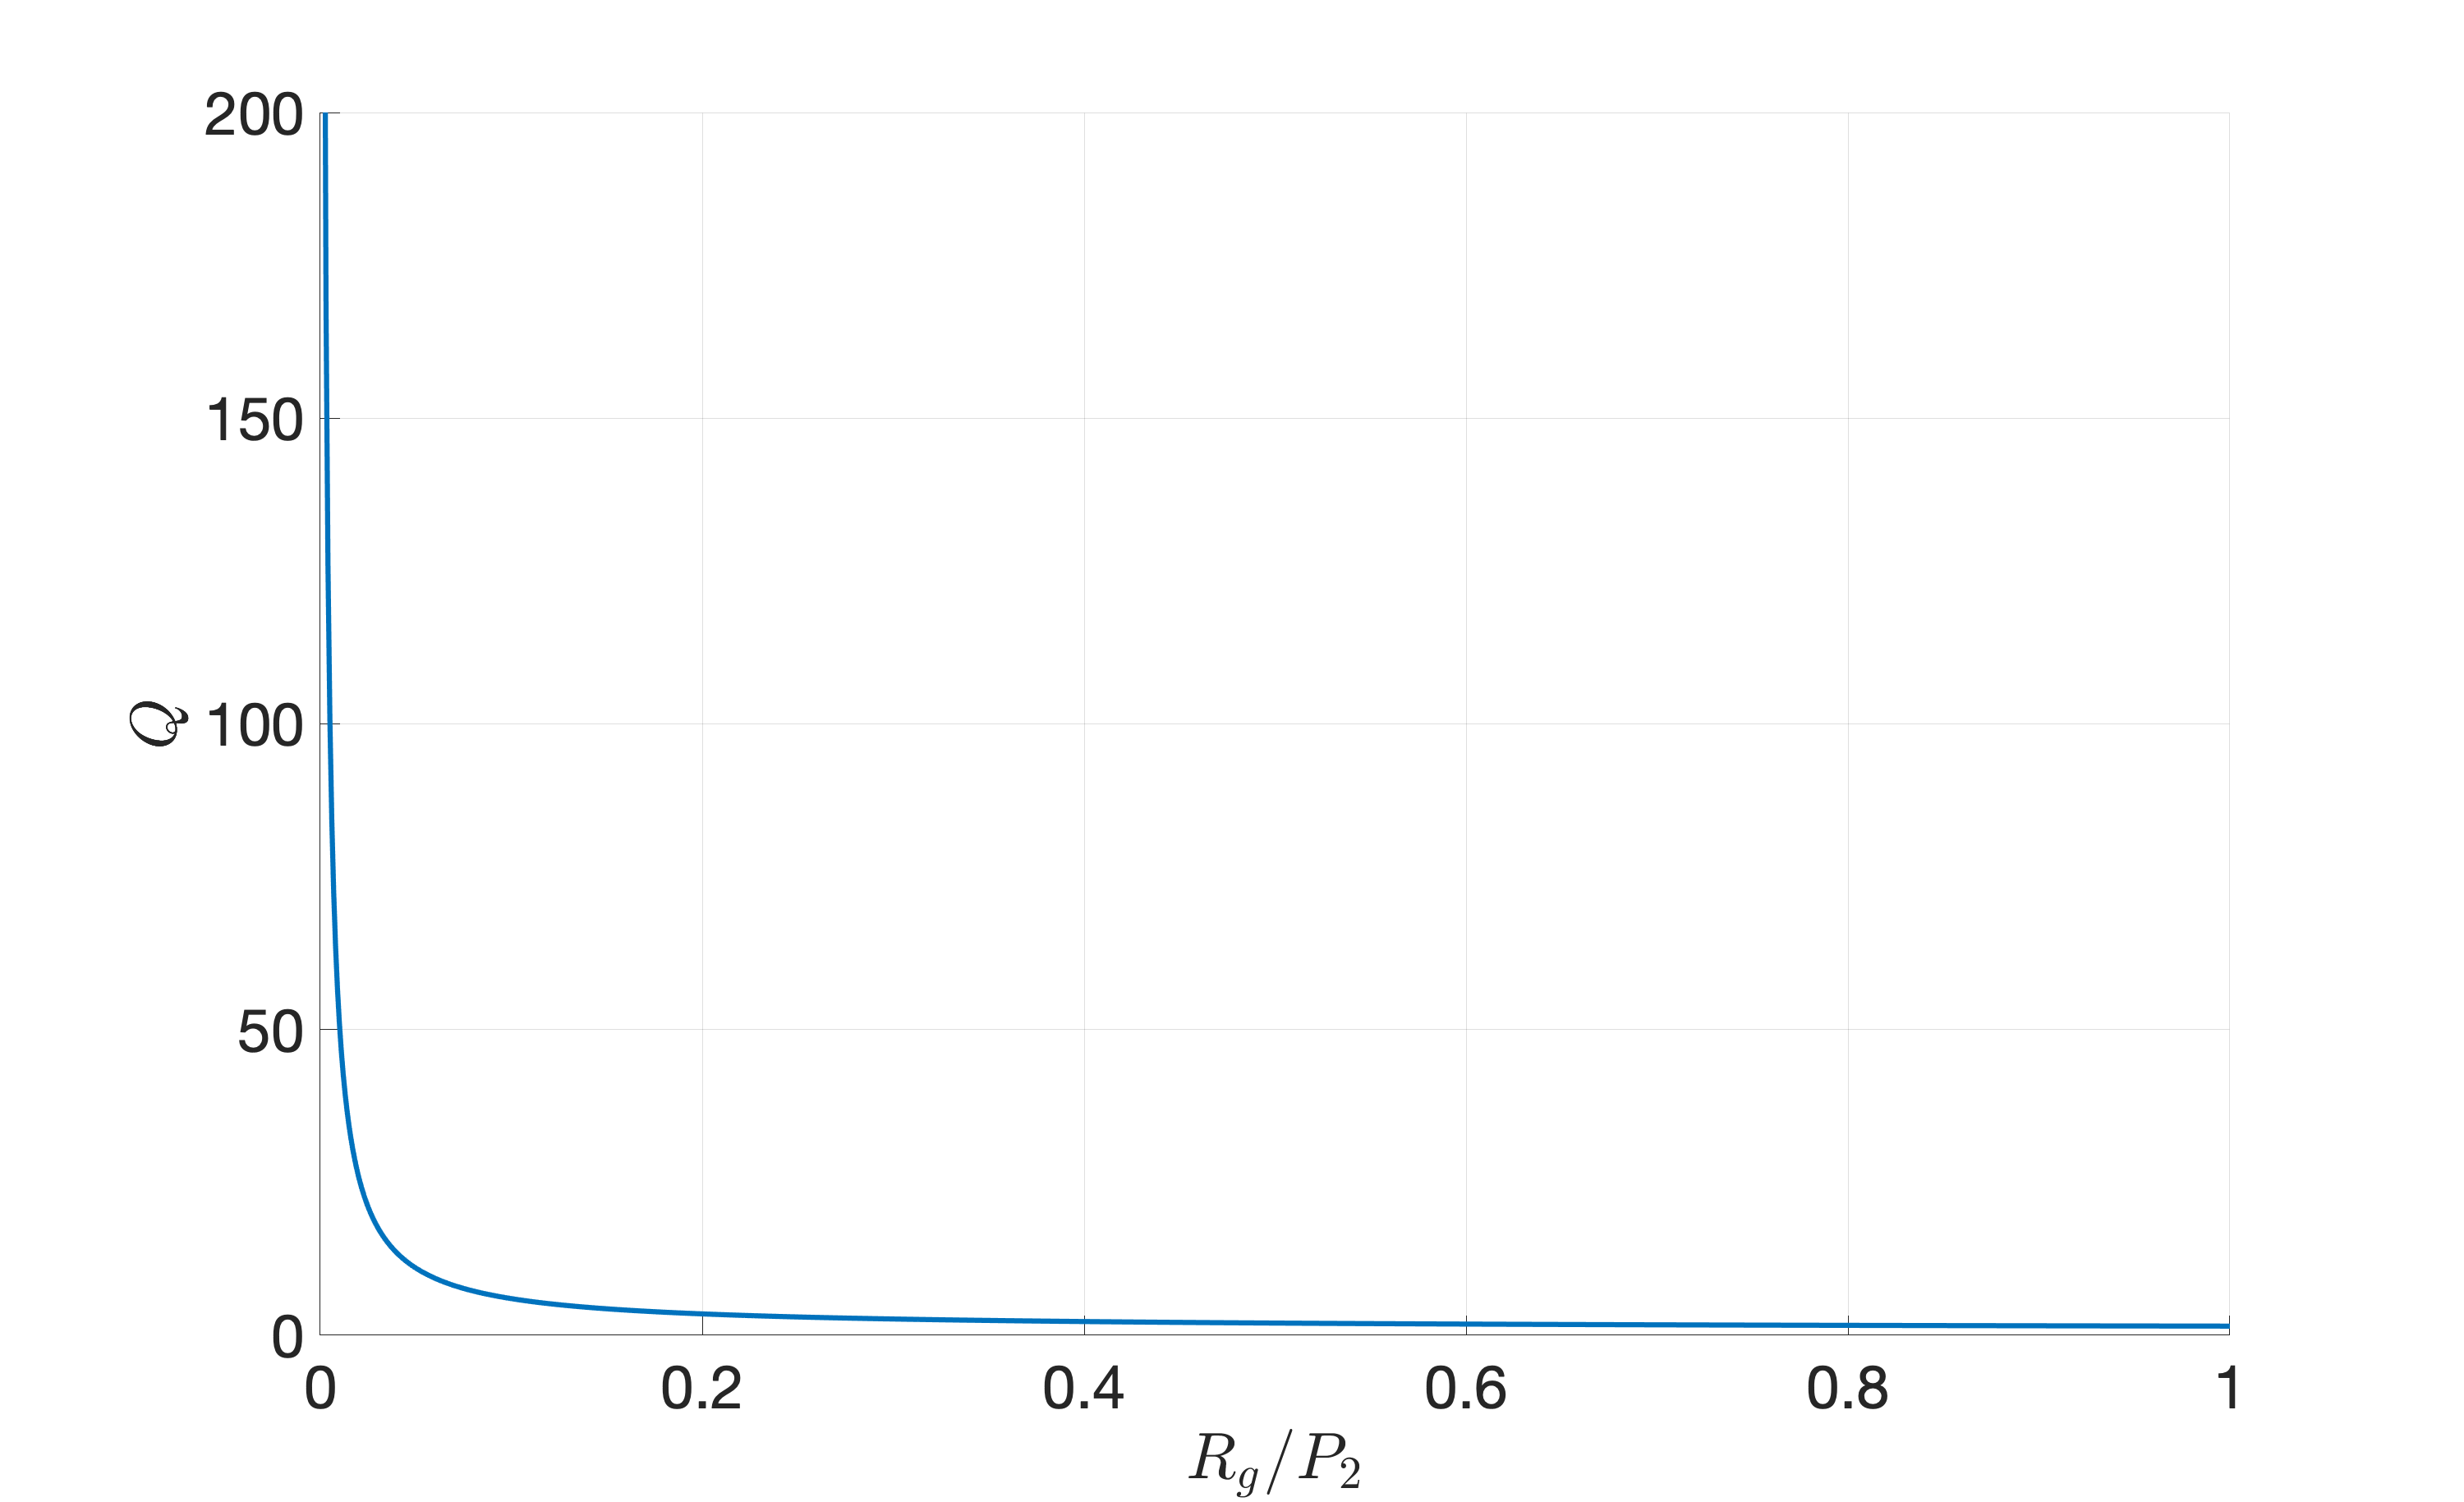
\includegraphics[width=\textwidth]{Imagens/1_5_6_QPotentiometer3.png}
         \caption{Evolução de $Q$.}
     \end{subfigure}
    \caption{Evolução de $K$ e $Q$ com a posição do potenciómetro.}
    \label{fig:KQpot}
\end{figure}

\subsubsection{Trabalho Experimental}\label{sec:KNH_exp}
\vspace{2mm}
\noindent \textbf{2.1.2.1 \hspace{1mm}Identificação dos Filtros} \par
Depois de feita a montagem representada na Fig. \ref{fig:KHN}, o primeiro objetivo foi analisar o comportamento de cada saída do circuito ($V_1, V_2$, e $V_3$) e identificar tipo de filtro que cada uma representava. Para isso, para cada saída, foi analisado o seu comportamento para 3 frequências: uma baixa (500 Hz), uma média (3390 Hz) e uma alta (30 000 Hz). Primeiro, foi analisada a saída $V_1$, os resultados obtidos estão representados na Fig. \ref{saídas_v1}. Na Fig. \ref{saídas_v1} notamos que este filtro atenua baixas frequências, deixando passar frequências médias e altas. Este filtro é, portanto, um {filtro passa-alto}.

\begin{figure}[h!]
\centering
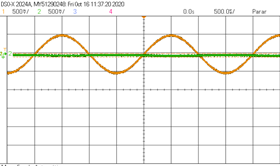
\includegraphics[width=.325\textwidth]{Imagens/v1_baixa_KNH.png}
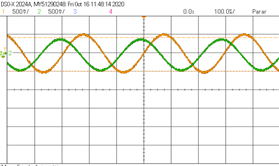
\includegraphics[width=.325\textwidth]{Imagens/v1_media.png}
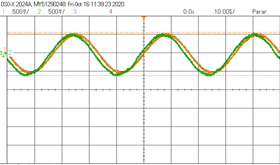
\includegraphics[width=.325\textwidth]{Imagens/v1_alta_KNH.png}
\caption{Saída $V_1$ para as frequências de 500Hz, 3390 Hz e 30kHz.}
\label{saídas_v1}
\end{figure}

Analisamos em seguida os resultados da saída $V_2$. Estes estão representados na Fig. \ref{saídas_v2}. Podemos observar que a saída $V_2$ atenua baixas frequências, não atenua frequências médias, e atenua também altas frequências. Trata-se então de um {filtro passa-banda}.

\begin{figure}[h!]
\centering
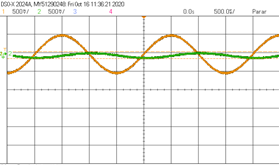
\includegraphics[width=.325\textwidth]{Imagens/v2_baixa_KNH.png}
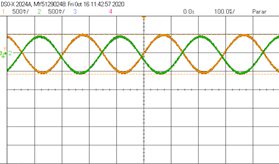
\includegraphics[width=.325\textwidth]{Imagens/v2_media_KNH.png}
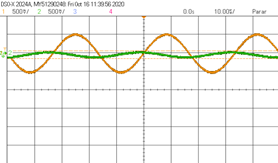
\includegraphics[width=.325\textwidth]{Imagens/v2_alta_KNH.png}
\caption{Saída $V_2$ para as frequências de 500Hz, 3390 Hz e 30kHz.}
\label{saídas_v2}
\end{figure}

Por último, os resultados da saída $V_3$ estão representados na Fig. \ref{saídas_v3}. Os resultados estão apresentados na Fig. \ref{fig:var_pot}. Este último filtro não atenua nem baixas, nem médias frequências, atenuando altas frequência. É, portanto, um {filtro passa-baixo}.

\begin{figure}[h!]
\centering
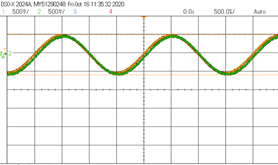
\includegraphics[width=.325\textwidth]{Imagens/v3_baixa_KNH.png}
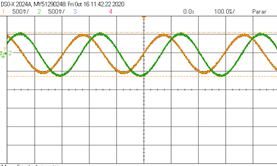
\includegraphics[width=.325\textwidth]{Imagens/v3_media_KNH.png}
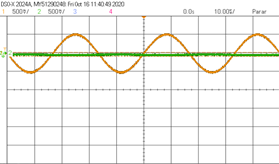
\includegraphics[width=.325\textwidth]{Imagens/v3_alta_KNH.png}
\caption{Saída $V_3$ para as frequências de 500Hz, 3390 Hz e 30kHz.}
\label{saídas_v3}
\end{figure}

\vspace{2mm}
\noindent \textbf{2.1.2.2. \hspace{1mm}Diagramas de Bode} \par
Para melhor compreender os resultados, recorreu-se ao uso de diagramas de Bode. Para tal, foi medida a amplitude pico-a-pico de saída, para um sinal de entrada de amplitude pico-a-pico constante, a diversas frequências. Optámos por escolher uma frequência baixa (0.5 $\si{\kilo \hertz}$), uma frequência alta (30 $\si{\kilo \hertz})$, e a frequência central do filtro passa-banda (3.79 $\si{\kilo \hertz}$), que foi determinada experimentalmente fazendo variar a frequência da onda de entrada até se verificar uma diferença de fase de $180\degree$. Foram ainda determinados dois pontos adicionais de modo a estudar a banda de passagem do filtro passa-banda. Partindo da frequência de corte, foram feitas duas medições, de modo a que a diferença de fase nessas medições correspondesse a $180\degree \pm 45\degree$. Apesar destes pontos adicionais serem particularmente relevantes para o filtro passa-banda, também foram utilizados para melhor compreender os diagramas de Bode dos filtros passa-baixo e passa-alto e comparar com os resultados esperados teoricamente. Foram então tiradas 5 medições para cada um dos filtros. Os resultados estão apresentados na Tabela \ref{tab:dados_bode_exp_KNH}.

\begin{table}[ht]
    \centering
    \caption{Valores experimentais das tensões de saída e dos ganhos da secção biquadrática KHN.}
    \begin{tabular}{cccccccc}
    \hline
        $f [\si{\kilo \hertz}]$ & $V_1 [\si{\volt}]$ & $T_1 (j \omega) [\si{\decibel}]$ & $V_2 [\si{\volt}]$ & $T_2 (j \omega)  [\si{\decibel}]$ & $V_3 [\si{\volt}]$ & $T_3 (j \omega) [\si{\decibel}]$ & $V_i[\si{\volt}] $\\
        \hline
        0.50   & 0.0400 & -28.7 & 0.145  & -17.5     & 1.10  & 0.0790  & 1.09\\
        2.30   &0.460 & -7.09 & 0.720  & -3.19     & 1.19  & 1.17  & 1.04\\
        3.79   &0.900 & -1.66 & 1.09  & 0.00     & 1.11  & 0.158 & 1.09\\
        6.20  &1.18 & 1.10 & 0.730  & -3.07     & 0.460  & -7.09  & 1.04\\
        30.00  &1.15 & 0.873 & 0.220  & -13.9    & 0.0270  & -32.1  & 1.09\\
    \hline
    \end{tabular}
    \label{tab:dados_bode_exp_KNH}
\end{table}
\par 

A partir dos dados obtidos podemos, assim, calcular os valores de $K$, $Q$, e $\omega_0$. O valor de $\omega_0$ é obtido facilmente através de 
\begin{equation}\label{eq:w0FiltKHN}
\omega_0 = 2\pi f_0\:,   
\end{equation}
fazendo uso da frequência de central do filtro passa-banda determinada experimentalmente como descrito acima.  Analisando as funções de transferências dos filtros \eqref{eq:tfKHN}, podemos verificar que para o filtro passa-baixo (saída $V_3$), para $f=0$, o ganho pode ser determinado por
\begin{equation}\label{eq:KLPFiltKHN}
    \left|\frac{V_3 (s)}{V_i (s)}\right| = K \:.
\end{equation}
A determinação dos valores experimentais calculados usando \eqref{eq:KLPFiltKHN} será designada de método 1. Alternativamente, para o filtro passa-baixo (saída $V_1$), para $f\rightarrow \infty$,
 o ganho pode ser determinado por
\begin{equation}\label{eq:KHPFiltKHN}
     \left|\frac{V_1(s)}{V_i (s)}\right| = K \:.
\end{equation}
A determinação dos valores experimentais calculados usando \eqref{eq:KHPFiltKHN} será designada de método 2.
Assim, usando os valores da frequência mais baixa ($f= 500$ Hz) e mais alta ($f = 30$kHz), respectivamente para o filtro passa-baixo usado o método 1 e para o filtro passa-alto usando o méotodo 2, podemos obter duas aproximações para o valor de $K$. No filtro passa-banda, para a frequência central $f_0$, o módulo do ganho é igual a 
\begin{equation}\label{eq:QFiltKHN}
    \left|\frac{V_2 (j\omega)}{V_i (j\omega)}\right|_{\omega = \omega_0} = KQ \implies Q =  \left|\frac{V_2 (j\omega)}{V_i (j\omega)}\right|_{\omega = \omega_0}/K\:,
\end{equation}
em que $K$ é calculado fazendo uso do método 1 ou 2, conforme descrito acima.
Utilizando \eqref{eq:w0FiltKHN}, \eqref{eq:KLPFiltKHN}, \eqref{eq:KHPFiltKHN}, e \eqref{eq:QFiltKHN}, é possível calcular os valores experimentais de $K$, $Q$, e $\omega_0$, apresentados na Tabela \ref{tab:comparação_resultados}.

\begin{comment}
Pela Tabela \ref{tab:dados_bode_exp_KNH}, quando $f_0 = 3.79 \si{\kilo\hertz}$,$\frac{V_2 (s)}{V_i (s)} = 1,00$, logo $Q=\frac{1}{K}= 0.990$ . \par
Para frequências altas, através de \eqref{eq:KHPFiltKHN} temos que $K=1.06$ e consequentemente que $Q=0.948$. O valor de $\omega_0$ é igual para os dois métodos utilizados.  Esta informação encontra-se resumida na Tabela \ref{tab:comparação_resultados}.
em que $f_0=3.79 kHz$ é a frequência de corte.
 Logo $\omega_0 = 2.38 \times 10^4 \si{\radian\per\second}$.
 temos que \textbf{$K=1.01$}.
\end{comment}

Alternativamente, também se optou por calcular $K, Q$, e $\omega_0$ através de um método de mínimo quadrados, adaptando a curva do filtro passa-banda, $|T_2 (j\omega)|$ com função de transferência descrita em \eqref{eq:tfKHN}, aos dados experimentais obtidos. Obteve-se, assim, a curva representada na Fig. \ref{regressão_KHN} e os valores de $K, Q$, e $\omega_0$ apresentados na Tabela \ref{tab:comparação_resultados}. Este é designado de método 3.

\begin{figure}[h!]
    \centering
    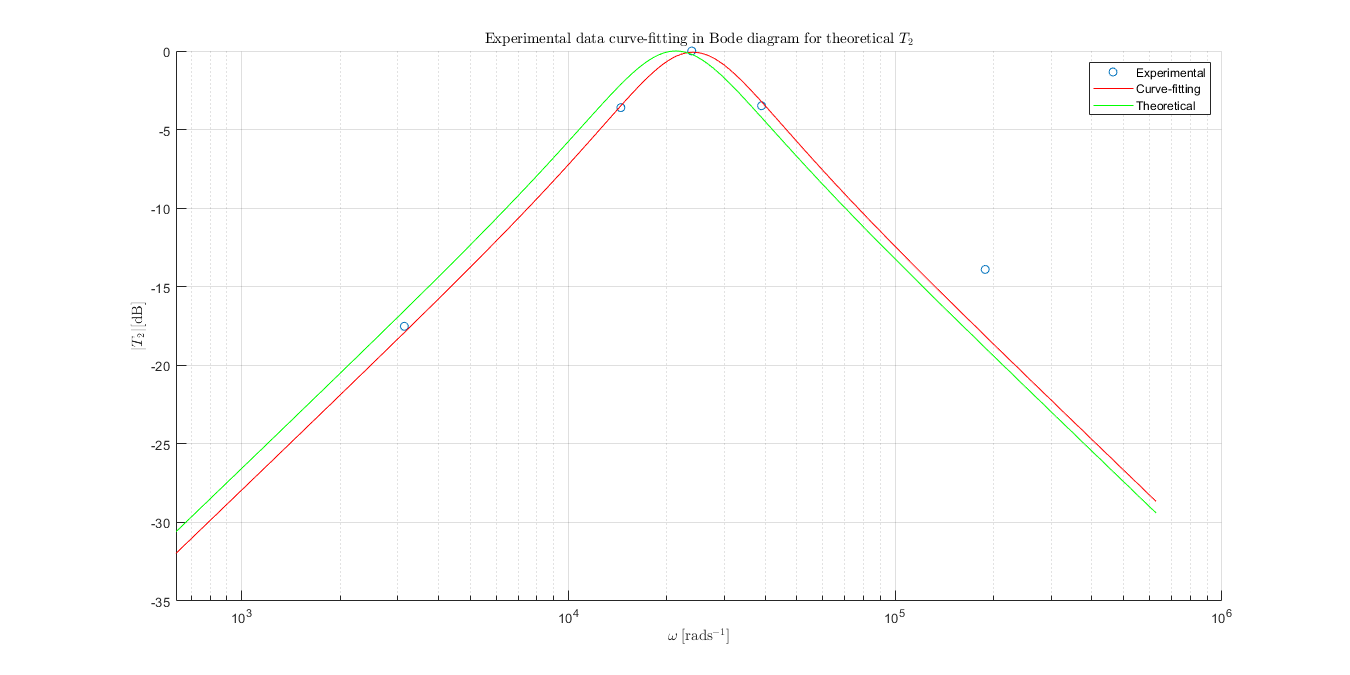
\includegraphics[width = 0.8\textwidth]{Imagens/regressao_passabanda.png}
    \caption{Adaptação de uma curva de acordo com $T_2$ teórica aos resultados experimentais.}
    \label{regressão_KHN}
\end{figure}

\vspace{2mm}
\noindent\textbf{2.1.2.3 \hspace{1mm}Potenciómetro como divisor de tensão} \par
Na última parte do laboratório, alterámos o circuito de modo a que $P_2$ funcionasse como divisor de tensão variável. Temos como objetivo determinar o efeito da variação deste divisor sobre as características de resposta em frequência da secção biquadrática de KHN. Em primeiro lugar, foi medido o valor de $P_2$, de modo a poder comparar com o valor nominal disponibilizado no enunciado. Em segundo lugar, a partir do valor de $P_2$ determinado experimentalmente e, tendo em conta \eqref{eq:rv_rg} e a montagem representada na Fig. \ref{fig:KNH_pot}, variámos o valor de $R_g$ para os valores apresentados na Tabela \ref{tab:rg_variar}.

%\textcolor{purple}{MIUITO IMPORTANTE Valores de Rg mesmo do laboratótio -> refazer graficos teoricso com valores das resistencais Rg do lab}

\begin{table}[ht]
    \centering
    \caption{Medições de acordo a variação de $R_g$.}
    \begin{tabular}{cccccc}
    \hline
        $R_g$ Medido [k\ohm] & $R_g$ Pretendido [k\ohm] & $f [Hz]$ & $V_3(s) [V]$ & $V_i (s) [V]$ & $|T_3 (j \omega)|[dB]$\\
        \hline
        1.968 & 2.014 & 100 & 0.360 & 1.11& -9.78\\
        1.968 & 2.014 & 3790 & 0.980 & 1.11&-1.08 \\
        7.872 & 7.800 & 100 & 0.380 & 1.11& -9.31\\
        7.872 & 7.800 & 3790 & 0.300    & 1.11& -11.4\\
        3.936 & 3.950 & 100 & 0.480 & 1.09&-7.12 \\
        3.936 & 3.950 & 3790 & 0.700 & 1.11 & -4.00\\
        5.904 & 5.890 & 100 & 0.480 & 1.09&-7.12 \\
        5.904 & 5.890 & 3790 & 0.520 & 1.11& -6.59 \\
        
    \hline
    \end{tabular}
    \label{tab:rg_variar}
\end{table}

\begin{table}[ht]
    \centering
    \caption{Medição de $P_2$ e comparação com valor nominal.}
    \label{tab:P2_teo_exp}
    \begin{tabular}{cc}
    \hline
        $P_2$ nominal $[k\ohm]$ & $P_2$ experimental $[k\ohm]$ \\
        \hline
        10.0& 9.84 \\
    \hline
    \end{tabular}
\end{table}


%Tabela teste \par
%\begin{table}[]
%\begin{tabular}{lllll}
%\multicolumn{2}{l}{\multirow{2}{*}{1}} &  &  &  \\
%\multicolumn{2}{l}{} &  &  &  \\
%\multicolumn{2}{l}{\multirow{2}{*}{2}} &  &  &  \\
%\multicolumn{2}{l}{} &  &  &  \\
%\multicolumn{2}{l}{\multirow{2}{*}{3}} &  &  &  \\
%\multicolumn{2}{l}{} &  &  &  \\
%\multicolumn{2}{l}{\multirow{2}{*}{4}} &  &  &  \\
%\multicolumn{2}{l}{} &  &  & 
%\end{tabular}
%\end{table}

\par
Para melhor compreender os resultados, recorremos ao uso de diagramas de Bode. Os resultados estão apresentados na Fig. \ref{fig:var_pot}. \par
\begin{figure}[h!]
    \centering
    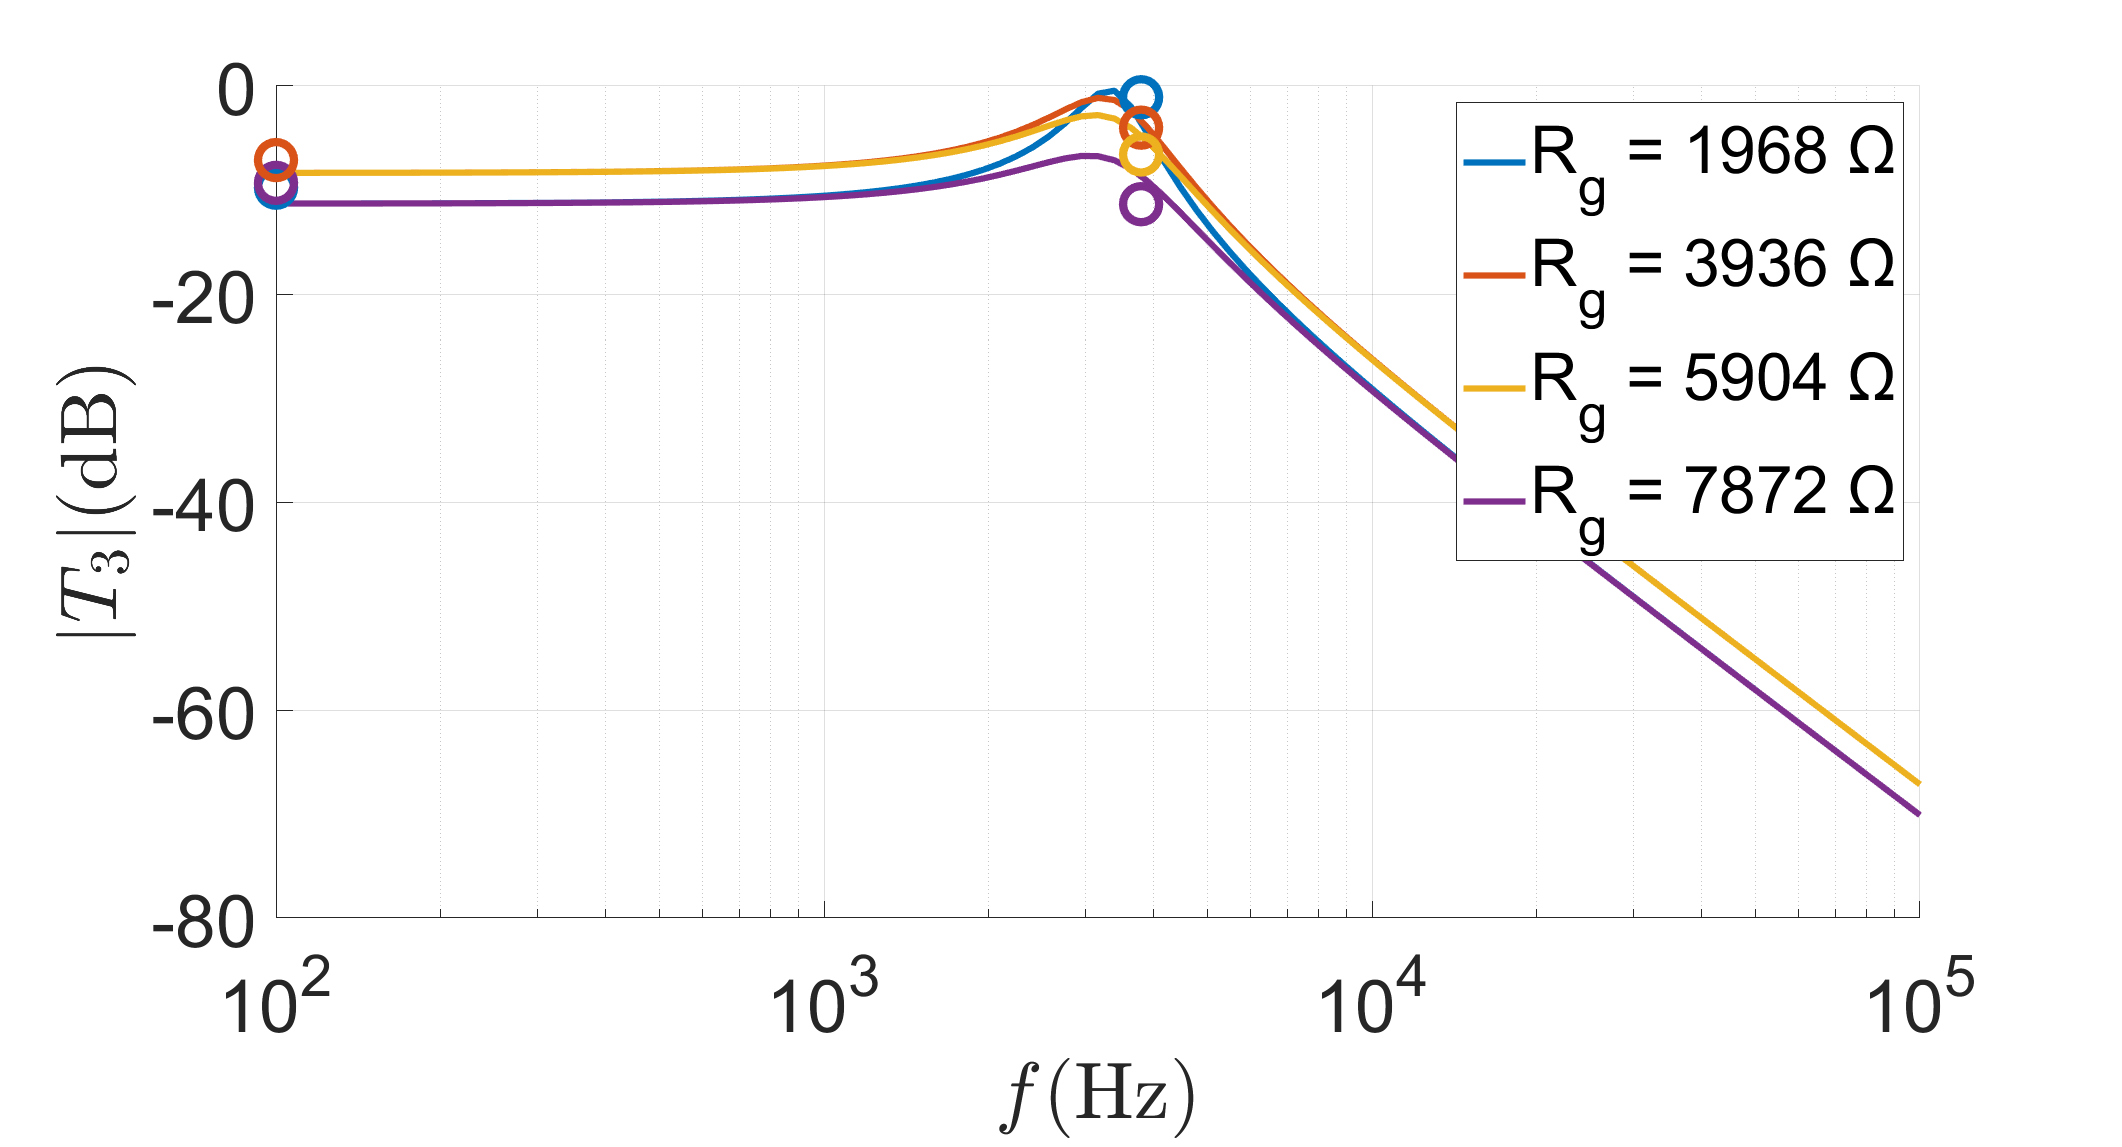
\includegraphics[width = 0.8\textwidth]{Imagens/1_5_6_bodeTheoreticalPotentiometer3.png}
    \caption{Diagrama de Bode para $R_g$ variável.}
    \label{fig:var_pot}
\end{figure}
\par

%Uma vez que as resistências $R_v$ e $R_g$ são complementares, devemos analisar as retas representadas aos pares. Temos então o primeiro par: $R_g=1968 k\ohm$  e $R_g=7872 k\ohm$ (azul e roxo na Fig. \ref{fig:var_pot}), e o segundo par $R_g=3936k\ohm$ e $R_g=5904 k\ohm$ (laranja e amarelo na Fig. \ref{fig:var_pot}). Pela figura, em primeiro lugar podemos concluir que o valor de $K$ para cada par de retas é constante, corroborado pela sobreposição das retas para baixas frequências. Em segundo lugar, analisando o gráfico na zona da frequência de corte, concluímos que o parâmetro alterado é $Q$, sendo que nesta frequência o valor de $Q$ vai diminuindo com o aumento do coeficiente de $R_g$ em relação a $P_2$.\par

\subsubsection{Comparação de Resultados}
Pela análise teórica, concluímos que as saídas $V_1$, $V_2$, e $V_3$ funcionariam como filtros passa-alto, passa-banda e passa-baixo, respetivamente, o que foi verificado durante a obtenção de dados do procedimento experimental. No que diz respeito à análise dos diagramas de Bode, cuja comparação entre os valores teóricos e os pontos experimentais tirados está representada na Fig. \ref{fig:bode_exp_KNH_comentar}, os resultados obtidos são os esperados.

Para complementar esta informação, foi calculado também a variação assintótica do ganho de cada tipo de filtro, para baixas e altas frequências (quando relevante), por forma a determinar a ordem dos filtros experimentalmente. Para calcular estes declives foi feita uma regressão linear com os dois pontos de menor frequência correspondentes a cada gráfico (para calcular o ganho por década a baixas frequências para $T_1$ e $T_2$) e com os dois pontos de maior frequência correspondentes a cada gráfico (para calcular o ganho por década para altas frequências para $T_2$ e $T_3$). Os resultados estão apresentados na Tabela \ref{tab:ganhos}. \par
\begin{figure}[ht]
     \begin{subfigure}[b]{0.45\textwidth}
         \centering
         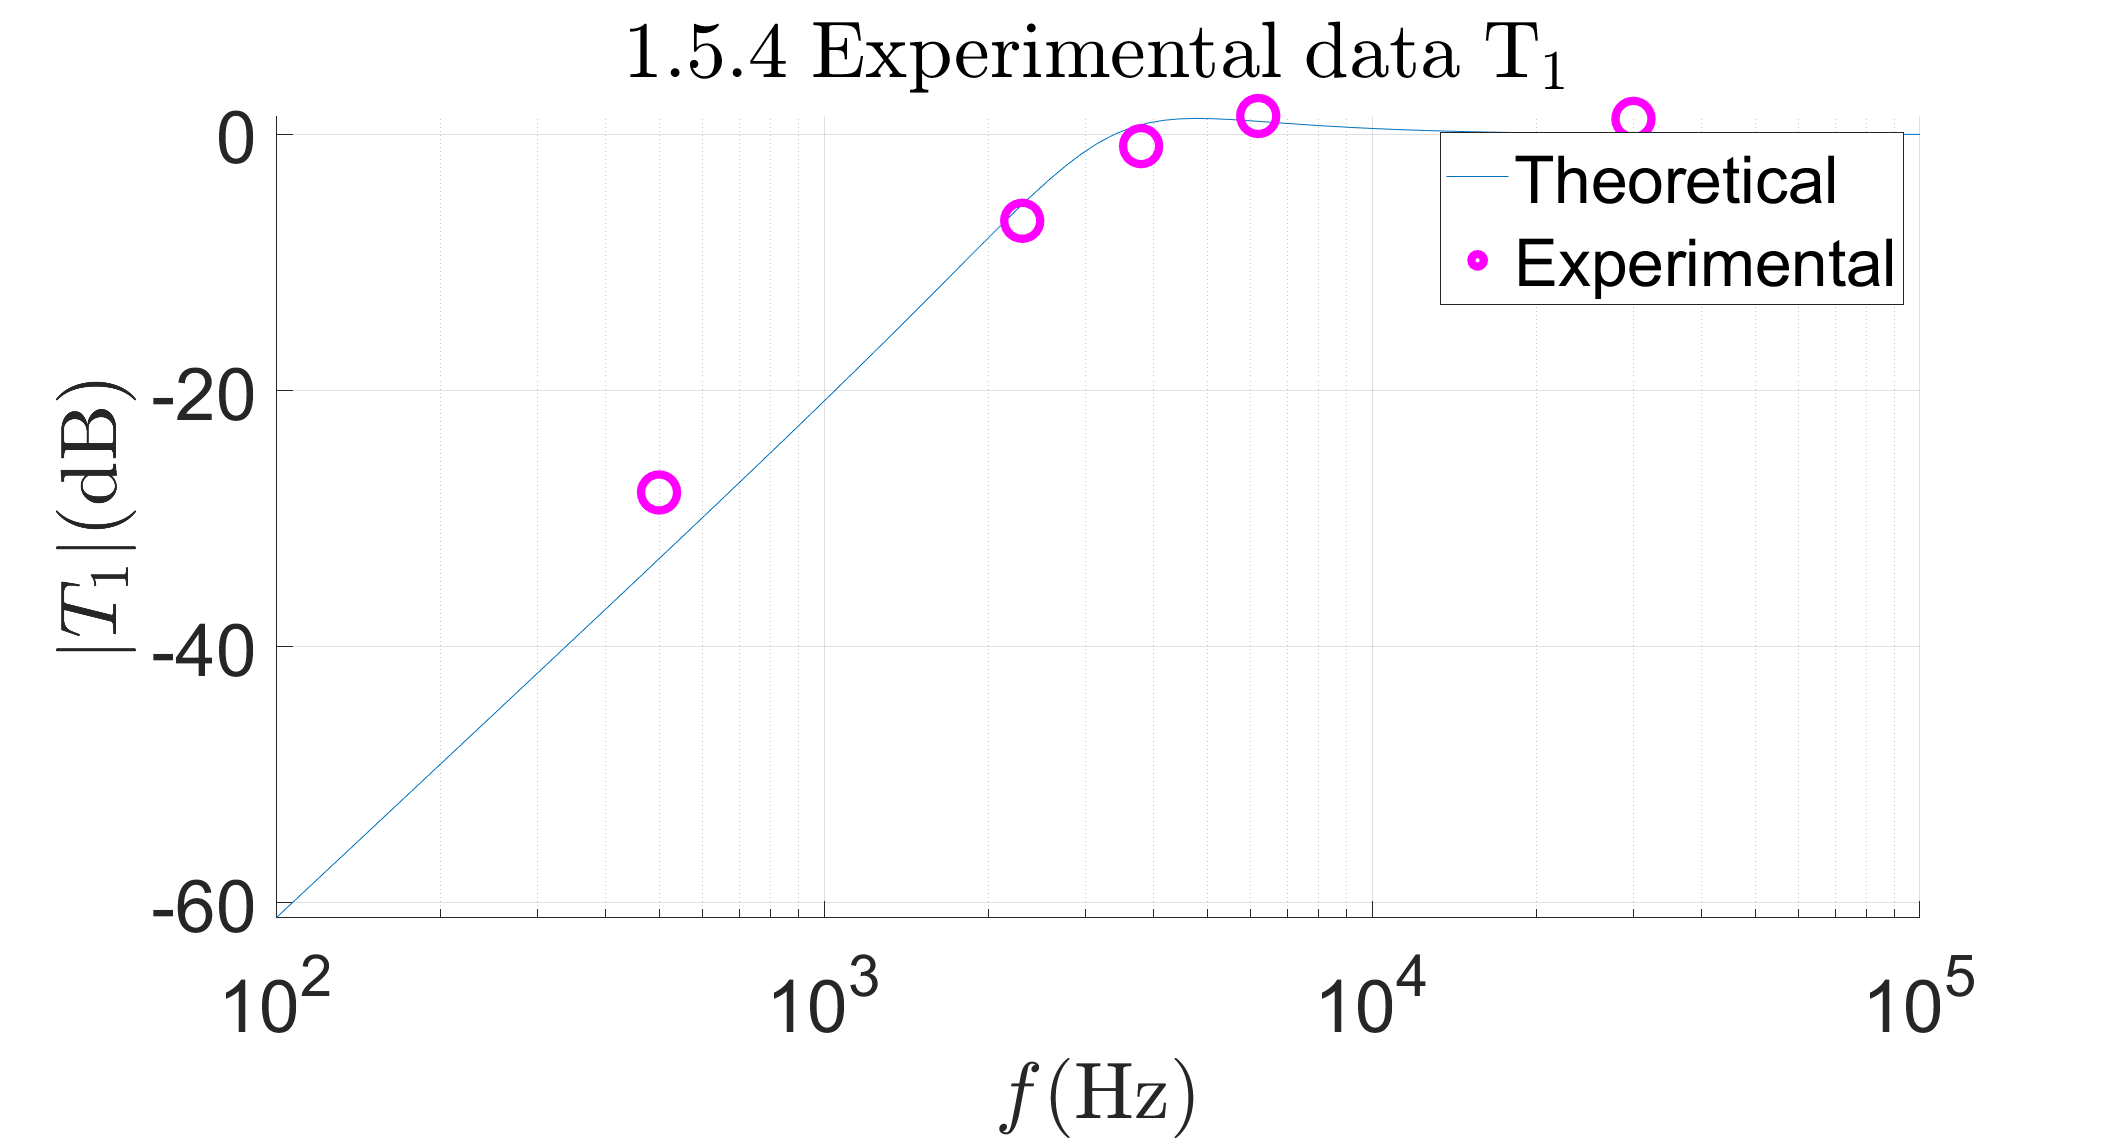
\includegraphics[width=\textwidth]{Imagens/1_5_4_bodeExperimental1.png}
         \caption{Filtro $T_1$}
         \label{fig:bode_exp_KNH_comentar_T1}
     \end{subfigure}
     \hfill
     \begin{subfigure}[b]{0.45\textwidth}
         \centering
         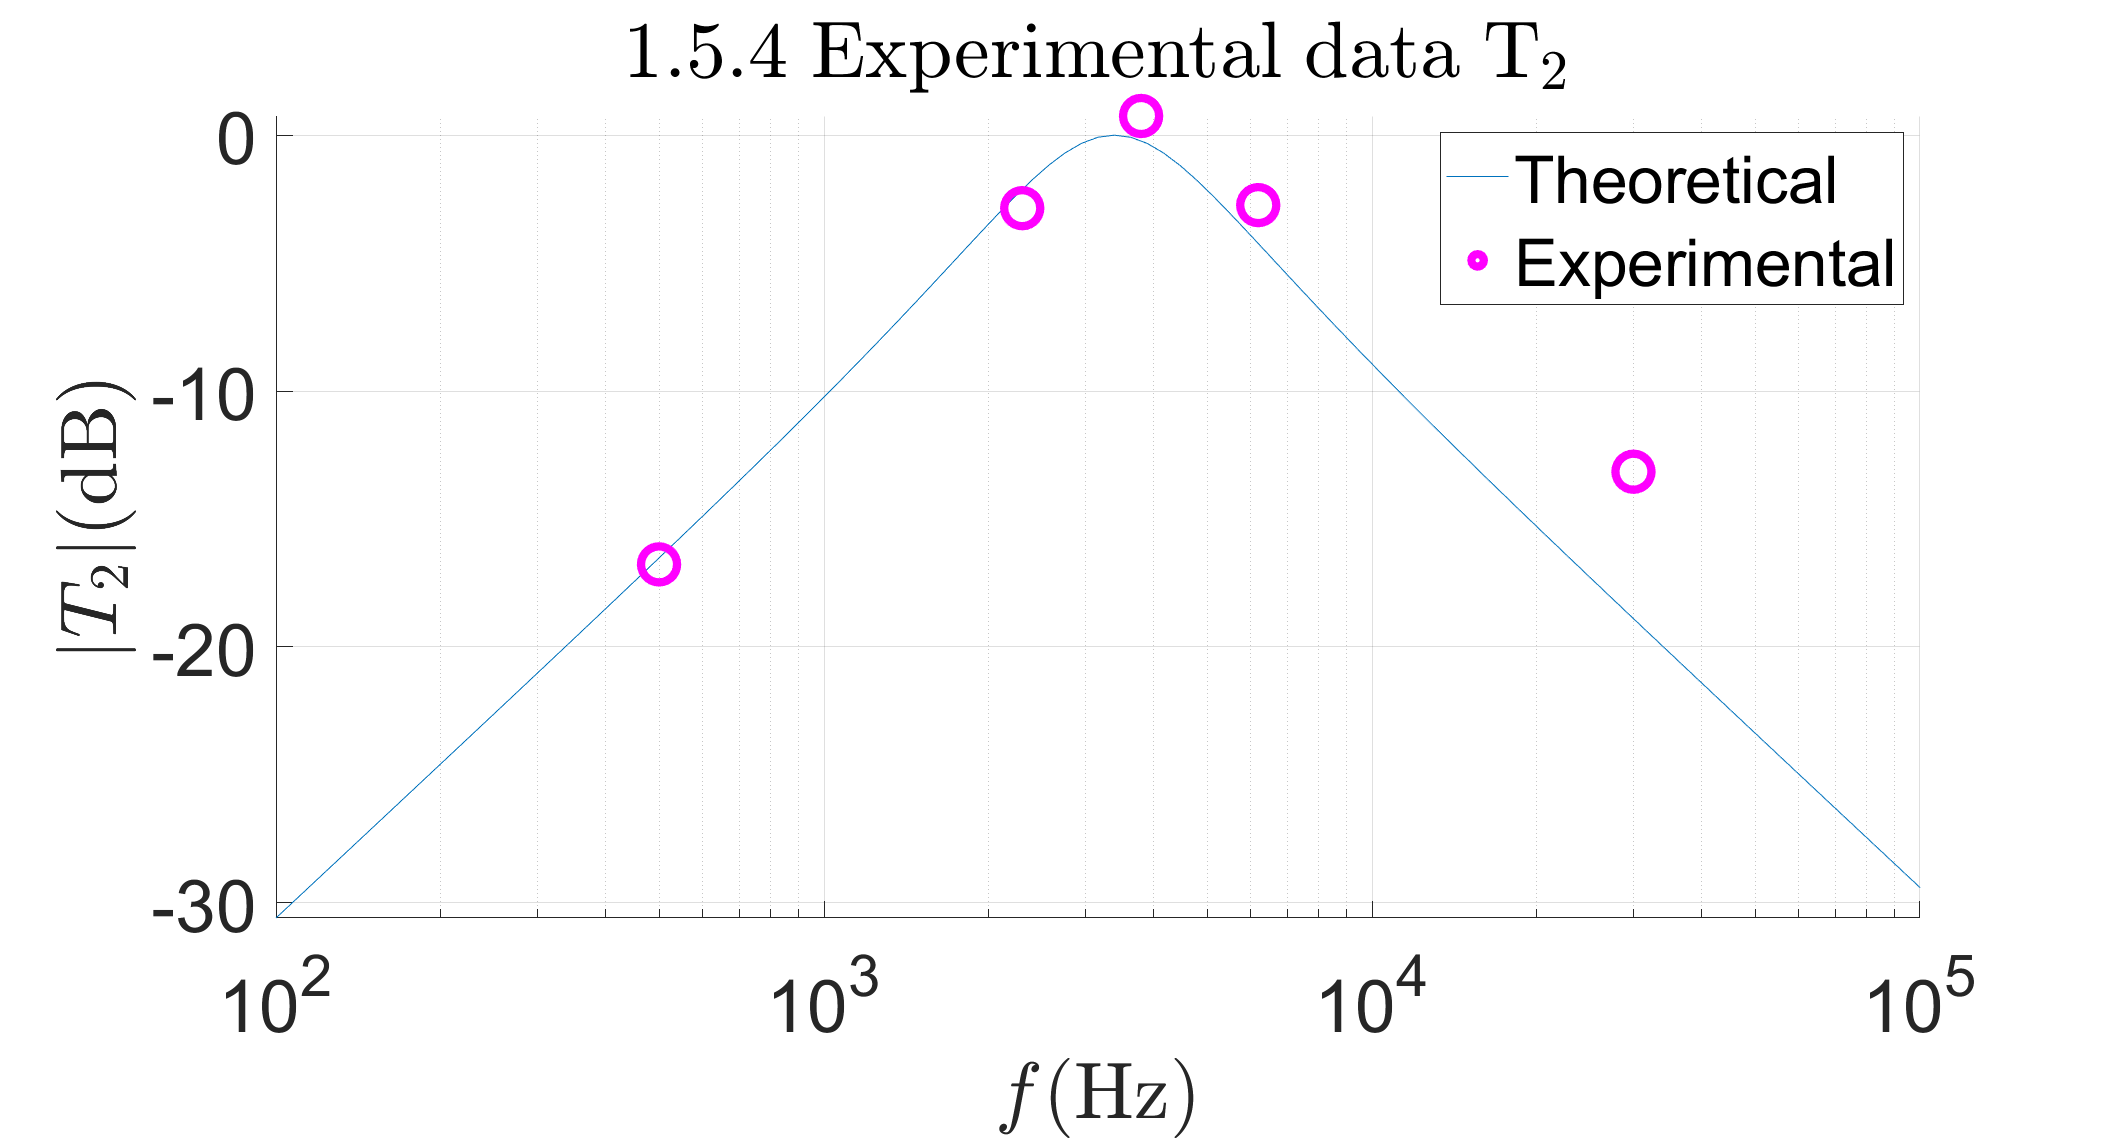
\includegraphics[width=\textwidth]{Imagens/1_5_4_bodeExperimental2.png}
         \caption{Filtro $T_2$}
         \label{fig:bode_exp_KNH_comentar_T2}
     \end{subfigure}
     \begin{subfigure}[b]{0.45\textwidth}
         \centering
         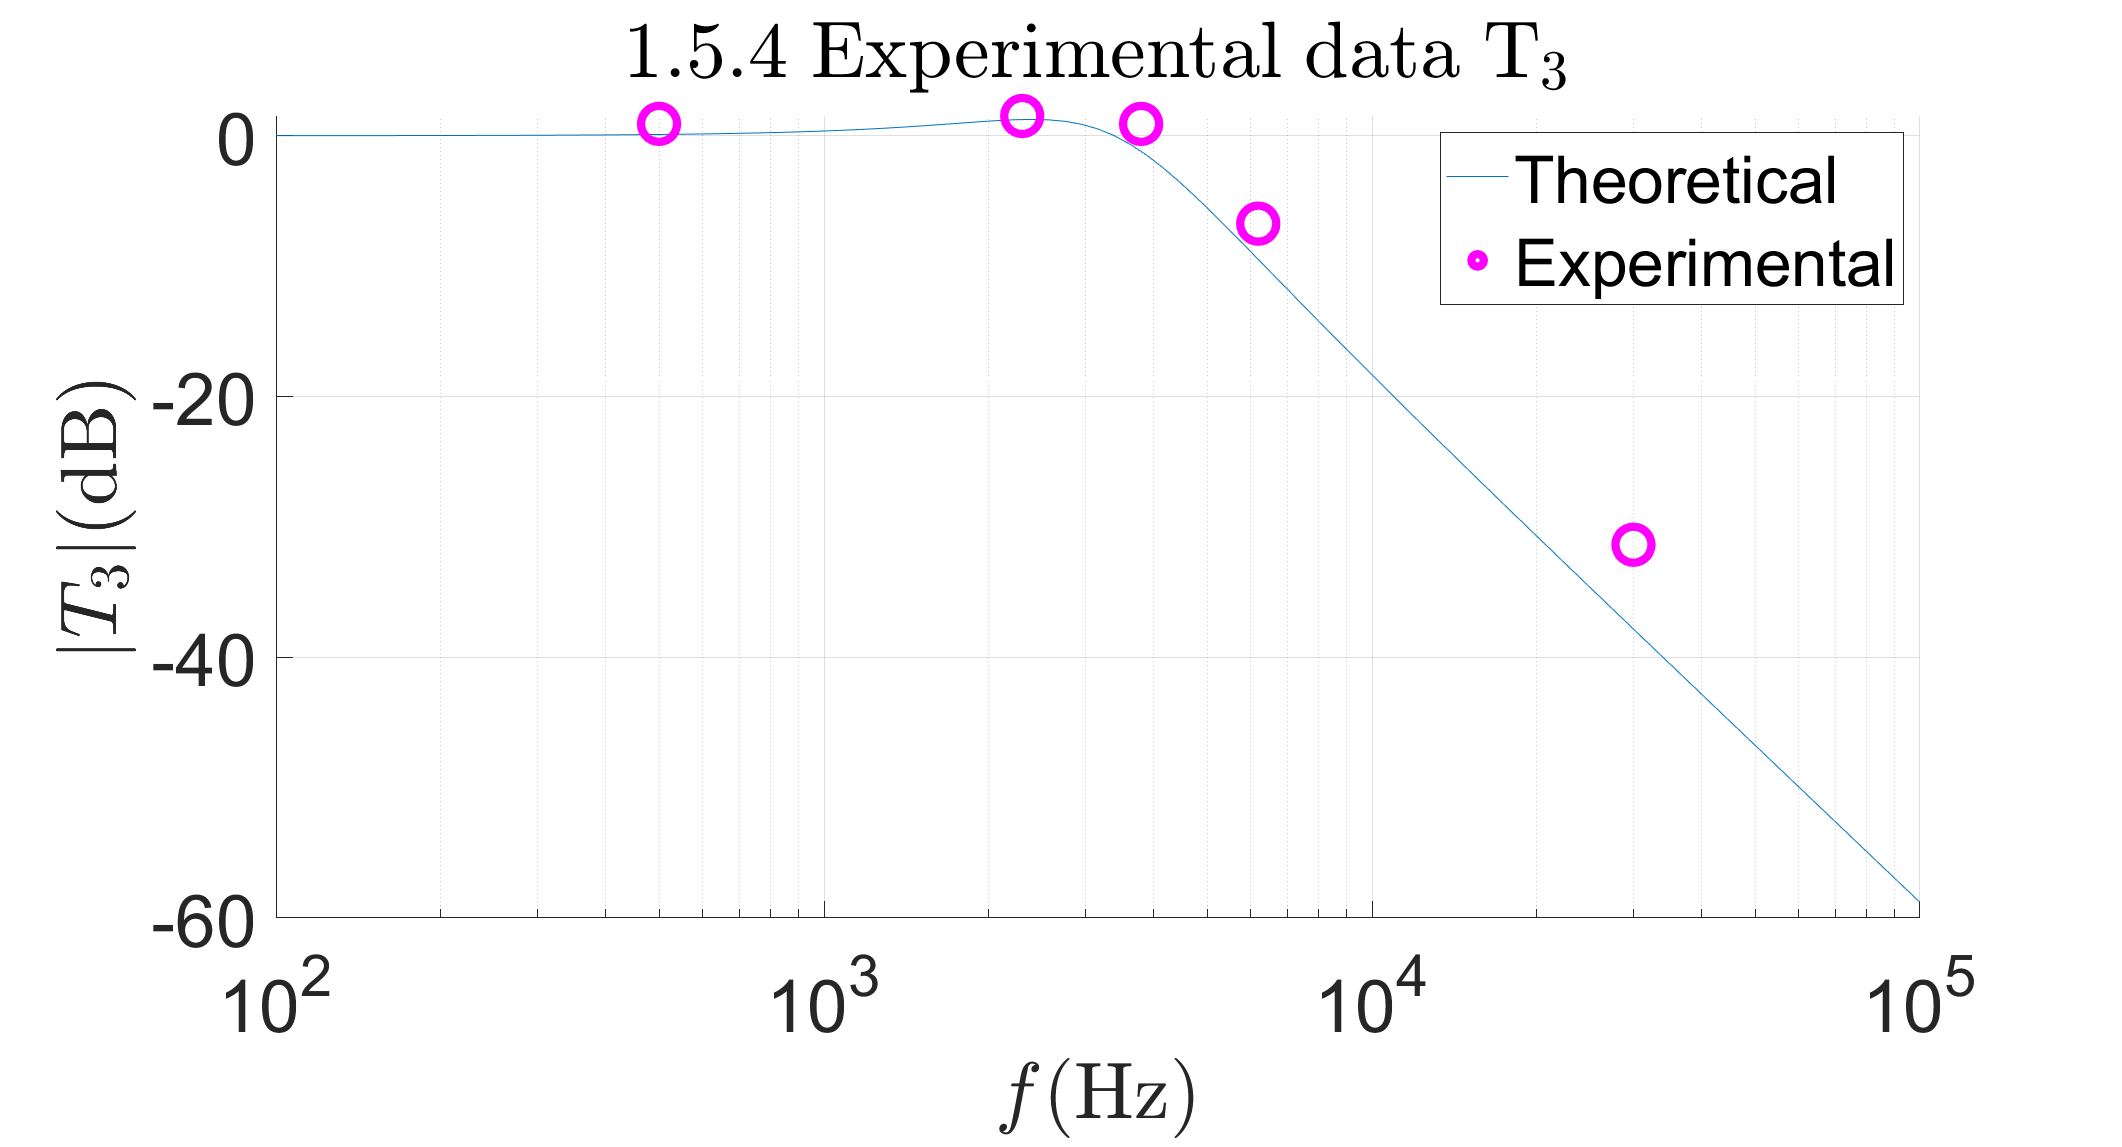
\includegraphics[width=\textwidth]{Imagens/1_5_4_bodeExperimental3.png}
         \caption{Filtro $T_3$}
         \label{fig:bode_exp_KNH_comentar_T3}
     \end{subfigure}
    \hfill
    \caption{Diagramas de Bode de amplitude teóricos e experimentais}
    \label{fig:bode_exp_KNH_comentar}
\end{figure}
\par

Em primeiro lugar, para $T_1$, os pontos obtidos experimentalmente, estão na vizinhança da curva teórica, sendo portanto representativos do filtro passa-alto já que mostram um ganho/década positivo a baixas frequências e um ganho praticamente nulo a partir da frequência de corte . Em segundo lugar, para $T_2$ o filtro passa-banda, apesar de um ligeiro deslocamento dos pontos em relação ao gráfico teórico, este deslocamento é coerente com a forma de onda esperada, sendo, portanto, os resultados satisfatórios. Finalmente, para o filtro passa-baixo, $T_3$, os pontos também se adequam bem ao gráfico teórico. Para além do ganho/década negativo a altas frequências, também é possível reparar que a baixas frequências e até à frequência de corte, os pontos medidos apresentam um ganho aproximadamente nulo, como característico de um filtro passa-baixo. 

Em quarto lugar, podemos observar que os erros associados aos declives calculados com a regressão linear são bastante altos. É para $T_1$, o filtro passa-alto, para baixas frequências, que se observa o maior erro em relação à variação assimptótica esperada. No entanto, uma vez que a regressão linear para calcular o ganho por década foi só feita com os 2 pontos disponíveis para cada situação, podemos admitir que uma grande componente do erro advém deste facto. Caso tivéssemos um maior número de pontos disponíveis a aproximação seria melhor já que, observando os gráficos da Fig. \ref{fig:bode_exp_KNH_comentar} , podemos concluir que todos os pontos obtidos se encontram na vizinhança da curva teórica. É também de salientar que alguns dos erros estão sempre associados aos componentes eletrónicos uma vez que os seus valores experimentais diferem dos valores nominais devido à tolerância que estes mesmos componentes apresentam. No entanto, apesar de os ganhos por década experimentais calculados terem bastante erro associado, estes conseguem corroborar a ordem dos filtros teoricamente prevista, tratando-se, assim, todos de filtros de 2ª ordem. 


%, este ganho é anulado por 2 pólos colocados à frequência de corte, tornando assim o ganho aproximadamente 0 dB a partir desta frequência .
%Para baixas frequências observa-se um ganho de cerca de 21.6dB/década, para altas frequências o ganho é de cerca de -15.8dB/década, os valores esperados seriam 20dB/década e -20dB/década respetivamente e portanto os erros associados são 8\% e -21\%. 
%sendo a queda a altas frequências -36.5dB/década, em relação -40 dB/década esperados, tendo então um erro associado de -8.75\%. 


\begin{table}[ht]
    \centering
    \caption{Comparação dos ganhos para cada filtro.}
    \begin{tabular}{cccc}
    \hline
         &Ganho Teórico [dB/década] & Ganho Experimental [dB/década] & Erro relativo (\%)\\
        \hline
        $T_1$ baixas frequências   & 40 & 32.6 &   -18.5\\
        $T_2$ baixas frequências   & 20 & 21.6 & 8.00 \\
        $T_2$ altas frequências   & -20 & -15.8 & -21.0 \\
        $T_3$ altas frequências   & -40 & -36.5 & -8.75 \\
    \hline
    \end{tabular}
    \label{tab:ganhos}
\end{table}

Analisando agora a frequência de corte para $T_1$ e para $T_3$. Em primeiro lugar, para $T_1$ e $T_3$ seria de esperar um ganho de -6.02dB para a frequência de corte, uma vez que estes são filtros passa-alto e passa-baixo, respetivamente, de 2ª ordem. No filtro passa-banda, à frequência central o ganho teórico é de 0dB e para as frequências de corte o ganho esperado é -3.01dB. Os valores experimentais deste ganhos, assim como os erros associados, são apresentados na Tabela \ref{tab:db_erros}. Como seria de esperar, os resultados melhores são os do filtro passa-banda uma vez que as frequências de corte e a frequência central foram determinadas analisando a resposta experimental deste mesmo filtro.

\begin{table}[ht]
\caption{Ganho nas frequências de corte e frequência central.}
    \centering
    \begin{tabular}{cccc}
    \hline
        Parâmetro & Valor Teórico[dB] & Valor Experimental[dB] & Erro relativo(\%)  \\
        \hline
         $T_1, f=2300 Hz$ & -6.02 & -7.09 & 17.8 \\
         $T_3, f=6200 Hz$ & -6.02 & -7.09 & 17.8 \\
         $T_2, f=3790 Hz$ & 0.00 & 0.00 & 0.00 \\
          $T_2, f=2300 Hz$ & -3.01 & -3.19 & 5.98 \\
           $T_2, f=6200 Hz$ & -3.01 & -3.07 & 1.99 \\
           \hline
    \end{tabular}
    
    \label{tab:db_erros}
\end{table}
\par

Passamos agora à análise entre os valores de $K$, $Q$, e $\omega_o$ teóricos e os valores calculados experimentalmente. A informação recolhida encontra-se representada na Tabela \ref{tab:comparação_resultados}. O maior erro foi o erro associado à frequência de corte. Este erro é principalmente devido à tolerância dos componentes eletrónicos, especialmente dos condensadores. Também é de salientar que na determinação do valor da frequência de corte experimentalmente é introduzido um erro de medição significativo, já que os valores das saídas muitas vezes não são constantes, acabando por flutuar entre uma gama de valores, tornando a determinação precisa da frequência de corte mais difícil. Por outro lado, tanto para $K$ como para $Q$ os resultados obtidos têm erros relativos muito baixos para o método 1 e erros relativos também baixos, mas superiores aos do método 1 para o método 2 e 3. Podemos concluir que o método 1 foi o método que obteve os resultados mais próximos dos teóricos.

\begin{table}[ht]
    \centering
    \caption{Comparação entre os valores teóricos de K,Q e $\omega_0$}
    \begin{tabular}{cccccccc}
    \hline
         & Teórico & Método 1 & Erro (\%) & Método 2 & Erro (\%) & Método 3 &Erro (\%)\\
        \hline
        $K$   & 1.00 & 1.01 &  1.00  & 1.06 & 6.00 & 0.964 & -3.6 \\
        $Q$   & 1.00 & 0.990 & -1.00 & 0.948 & -5.20 & 1.03 & 3.00 \\
        $\omega_0$   & $2.128 \times 10^4$ & $2.381 \times 10^4$ & -10.6 & $2.381 \times 10^4$ & -10.6 & $2.400 \times 10^4$ & 12.8  \\
    \hline
    \end{tabular}
    \label{tab:comparação_resultados}
\end{table}

Passa-se agora à análise da influência de um divisor de tensão variável no circuito. Uma vez que as resistências $R_v$ e $R_g$ são complementares, iremos analisar as curvas representadas aos pares. O primeiro par é $R_g=1968 \ohm$  e $R_g=7872 \ohm$, apresentado a azul e roxo na Fig. \ref{fig:var_pot}, respetivamente, e o segundo par é $R_g=3936\ohm$ e $R_g=5904 \ohm$, apresentado a laranja e amarelo na Fig. \ref{fig:var_pot}, respetivamente. 

Comparando os pontos medidos da Tabela \ref{tab:rg_variar} com os pontos teóricos, podemos dividir a análise em: i) pontos a baixa frequência (500 Hz) e ii) pontos na frequência de corte (3790 Hz). A baixas frequências, o que pretendemos verificar é que $K$ é igual para cada par de curvas, o que acontece já que para $R_g=3.936 k\ohm$ e para $R_g = 5.904 k\ohm$ o ganho é igual e para $R_g=1.968 k\ohm$ e $R_g=7.872 k\ohm$ o ganho apresenta uma diferença pequena entre os dois valores. Para a análise na frequência de corte a premissa que se pretende comprovar é que $Q$ diminui com o aumento de $R_g$ para cada par de curvas com o mesmo $K$, \textit{i.e.}, para valores de $R_g$ complementares. Observando os valores do ganho experimentais para ambos os pares, verificamos que para cada par o ganho mais elevado é observado para o menor valor de $R_g$. Confirma-se assim que, de facto, para o mesmo valor de $K$ quanto maior for $R_g$ menor será o valor de $Q$. Os erros entre os valores experimentais e os valores teóricos são elevados, especialmente para a frequência de corte, visto que é uma zona com grande sensibilidade do ganho a variações do valor dos componentes em relação aos seus valores nominais. Ainda assim, consideramos que os resultados foram satisfatórios uma vez que conseguimos comprovar as relações qualitativas de $K$ e $Q$ com $R_g$, previstas na Fig. \ref{fig:KQpot}. 

\begin{table}[ht]
    \centering
    \caption{Comparação entre os valores teóricos e os valores experimentais do estudo da influência do divisior de tensão variável no circuito.}
    \begin{tabular}{cccc}
    \hline
         $R_g [k\ohm]$, $f[Hz]$ & Valor Experimental [dB] & Valor Teórico [dB]  & Erro relativo (\%)\\
        \hline
       1.968, 500 & -9.78 & -11.3 & -13.5 \\
        3.936,  500 & -7.12 & -8.35 & -14.7 \\
        5.904,  500 & -7.12 & -8.35 & -14.7 \\
        7.872,  500 & -9.31 & -11.3 & -13.5 \\
        1.968,  3790 & -1.08 & -3.55 &-69.6  \\
        3.936, 3790 & -4.00 & -3.35 & 19.4 \\
        5.904, 3790 & -6.59 & -4.82 & 36.7 \\
         7.872, 3790 & -11.4 & -8.68 & 31.3 \\
    \hline
    \end{tabular}
    \label{tab:erros_pot}
\end{table}
